%File: formatting-instruction.tex
\documentclass[letterpaper]{article}
\usepackage{aaai}
\usepackage{times}
\usepackage{helvet}
\usepackage{courier}
\usepackage{graphicx}
\usepackage{multicol}
\usepackage{natbib}
\usepackage{amsmath}
\frenchspacing
\setlength{\pdfpagewidth}{8.5in}
\setlength{\pdfpageheight}{11in}
\pdfinfo{
/Title (Insert Your Title Here)
/Author (Put All Your Authors Here, Separated by Commas)}
\setcounter{secnumdepth}{0}  
 \begin{document}
% The file aaai.sty is the style file for AAAI Press 
% proceedings, working notes, and technical reports.
%
\title{Formatting Instructions \\for Authors Using \LaTeX{}}
\author{AAAI Press\\
Association for the Advancement of Artificial Intelligence\\
2275 East Bayshore Road, Suite 160\\
Palo Alto, California 94303\\
}
\maketitle
\begin{abstract}
\begin{quote}
One of the main questions in the humanities is how cultures and artistic expressions changes over time. While a number of researchers have used quantitative methods to study changes in literature, music, and cinema, so far no one has applied computational techniques to analyze temporal development in any form of visual art. We propose a number of computational methods, including a novel method inspired by the distance correlation, for the analysis of temporal changes in artworks suitable for large datasets. We apply our techniques to a collection of 270,000 artworks created between 2000 and 2010 by users of the most well-known social network for non-professional art - DeviantArt. We compare artworks in two top level categories - Traditional Art and Digital Art - to see how the use of digital tools has influenced content and form of visual artworks during 2000-2010 period. Our analysis reveals a number of gradual and systematic visual and semantic changes over ten year period. Somewhat unexpectedly, our data shows that color features change at a greater rate for Traditional Art than Digital Art. Furthermore, because these artworks are classified by the creators into two general categories - Traditional Art and Digital Art - we are also able to study how the use of digital tools has influenced content and form of visual artworks during 2000-2010 period. 

\end{quote}
\end{abstract}

\noindent Over last year ten years, researchers in computer science, social computing and computational social science published tends of thousands of papers analyzing large social and cultural datasets using computational methods. The rise of social networks and media sharing sites in the middle of 2000s and the availability of their data  was the main catalyst for the growth of this research. However, the easy access to massive amounts of social media data also prevented scientists from considering certain questions that were central for social sciences and humanities in the 20th century: history and historical evolution Because of the newness of this data (Flickr, 2004-; YouTube, 2005-; Twitter, 2006-; Instagram, 2010-), it did not encourage the study social and cultural changes over long periods of time. Instead, they focused on the analysis of properties of social networks, the behaviors of their users and the relations between these behaviors and real-world phenomena (e.g, a well-known analysis by Google of the relations Google search queries and flu activity). When time was considered, typically it is on the scale of hours, days, months and in some rare cases a few years, but not decades. In other words, to use the terms of linguistics, computational study of social networks has focused on synchronic as opposed to diachronic dimensions (analysis of the system in a given moment rather than its evolution in time). While we gained in the granularity of information and much larger sample sizes was traded for the ability to study historical changes using pre-digital methods. 


\begin{figure}[h!]
    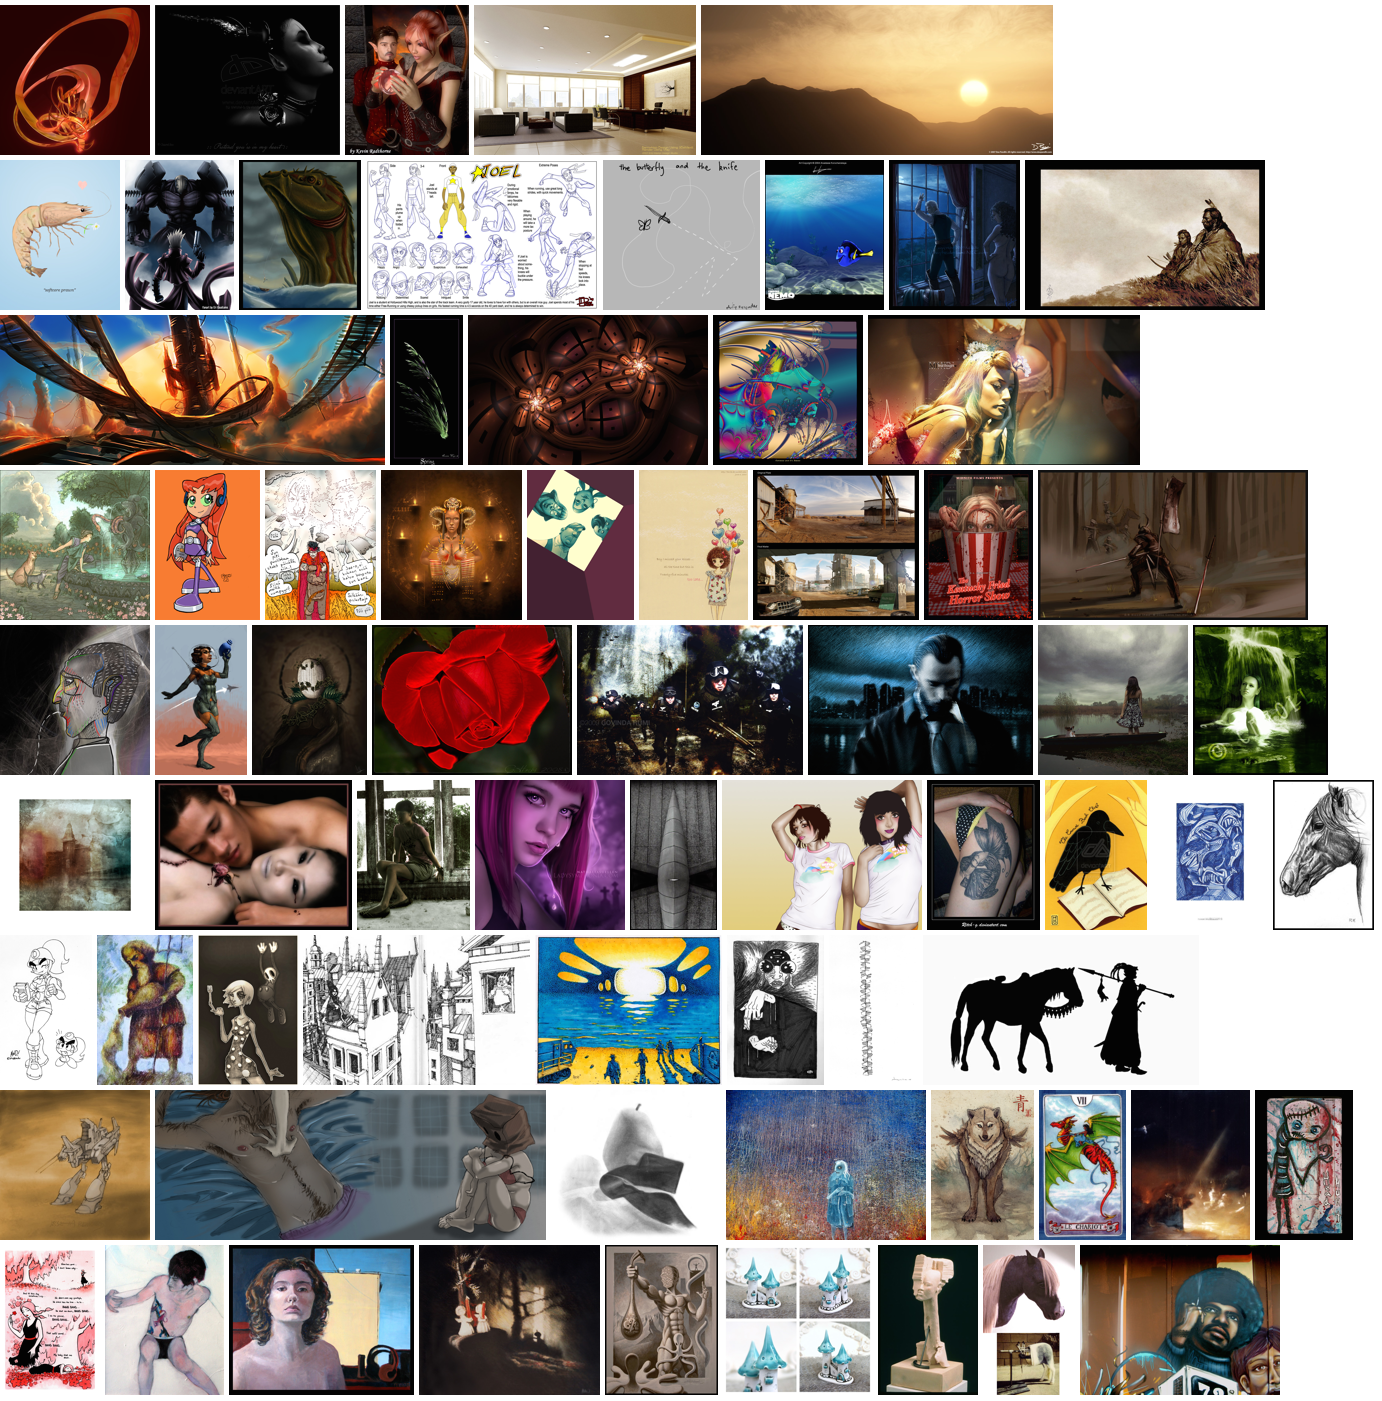
\includegraphics[width=0.5\textwidth]{top_20_percent_cats_1_images_each}
  \caption{A sample of deviantArt images representing the diversity of media and content. To create this sample, we selected 1 random image from each of top 20 percent of subcategories within Digital Art and Traditional Art categories.}
\end{figure}



One example is the use of data from Census surveys which in the U.S. were conducted since 1970. Another is longitudinal surveys that rely on repeated observations of the same variables over long periods of time. For instance, The 1970 British Cohort Study is a continuing longitudinal survey monitoring the development of 17,000 babies born in the UK in 1970 (the last survey was conducted in 2012).



	For humanities and social sciences, analyzing and explaining historical changes and differences between historical periods has been central since the formal founding of their various sub-disciplines in the second part of the 19th century. For example, let’s consider three founders of sociology: Karl Marx, Emile Durkheim, Max Weber. Karl Marx’s  economic theory postulated a number of different modes of production which replaced each other over the millennia. Emile Durkheim described evolution of societies as the move from “mechanical solidarity” to “organic solidarity,” while Max Weber proposed that the key differences between modernity and traditional societies were rationalisation, secularisation, and disenchantment. 
The very names of the large number of humanities fields indicate that they are concern with history. Besides the larger discipline of “history,” we have “art history,” “architectural history,” “history of photography,” “media history,” media archeology,” “music history,” “history of literature,” and so on. For example, to take just one discipline of art history, similar to the founders of sociology, the three founders of academic art history were keenly concerned with historical developments in the arts and crafts. Alois Riegl’s manuscripts of 1890s considered stylistic evolution across the entire history of western arts (“Historical grammar of the visual arts,” published posthumously). Heinrich Wölfflin’s "Principles of Art History" (1915) contrasted representations of forms in the 16th century and 17th century Italian art. Erwin Panofsky’s Perspective as Symbolic Form (1927) examined changes in the understanding and representation of spaces between Antiquity, Middle Ages and Renaissance.
Given the maturity of computational methods for the analysis of various media documents developed in digital image processing and computer vision, music information retrieval, computational linguistics and multimedia analysis fields, and the importance of historical analysis of changes in cultural artifacts, norms and behaviors for humanities, we would expect to see today massive research literature that applies these computational methods to digitized historical collections and also born-digital artifacts. In 2005 Manovich proposed such a research paradigm that he called “cultural analytics.” The goal of cultural analytics is study historical cultural development and contemporary culture using all existing digitized documents, born-digital artifacts, and all available social media and web data. In practice, since 2007 he and his collaborators focused on using techniques from computer vision to systematically study temporal patterns in variety of visual media, including art, photography, graphic design, comics, manga, web design, television programs, cartoons, motion graphics, use of illustrations in books and journals, etc. In 2010, the team of researchers from Harvard University and Google Books proposed a similar research program which they called “culturomics” - defined as the “ the application of high-throughput data collection and analysis to the study of human culture.” Their original research agenda was limited to the use of historical texts (e.g, five million digitized books from Google Books) but subsequently, Kalev Leetaru expanded this work to large text news archives including print and broadcast media. 
Surprisingly, with the exception of text analysis, such applications of computational methods to study historical changes in large cultural archives are still rare. We believe that there are three main reasons for this slowness of adaptation of computer methods to study historical changes in the arts. Firstly, computer scientists typically motivate their work with social networks data by references to practical applications (i.e., what already exists in the industry and is used by mass markets, such as search and recommendation). Therefore, they are unlikely to be interested in the study of cultural history, since this does not lead to any obvious mass markets opportunities. Secondly, among the humanities, only scholars of literature have used quantitative methods already since the 19th century, so they were prepared to switch from manually counting some characteristics in texts to using computers to do the same (first applications of computers for text analysis date from 1950s) .[chapter 1 of 1982 book on statistics for literary studies]. But the humanities scholars of non-textual cultural forms such as art, cinema, visual and audio media, dance, or architecture don’t have such tradition, and they are not yet aware that computers can be used to analyze content in cultural datasets. (As the result, the new field of “digital humanities” which started to rapidly grow in the second part of 2000s and which sees as one of its main goals quantitative computational analysis of massive cultural datasets so far is limited to analysis of literary texts). 
Thirdly, with the exception of literature, large high quality datasets of digitized historical works in other media have not yet been constructed. Typically image and media collections digitized by many libraries and archives are relatively small (<10,000 artifacts per collection), sparsely cover long historical period(s), do not come with APIs to facilitate their use by researchers, or only provide information about the artifacts (i.e., metadata), as opposed to the actual digitized artifacts. (A small number of exeptions which contains over 100,000 images as opposed to digitized texts and have APIs include a few digital collections in Library of Congress and in Digital Public Library of America http://dp.la/subjects, and Rijksmuseum API,). 
(For example of aps created with museum APIs, see )
	Most importantly, the typical digitized humanities collections are structurally different from social networks data used in social computing research. Networks such as Twitter, Facebook, or Instagram are both “broad” and “dense.” They are “broad” because they contain textual and visual expressions by hundreds of millions of people about infinite variety of topics. They are “dense,” because these expressions cover geo-spatial locations and moments in time with enough density to allow us to compare these locations and time periods. Of course, we have to always keep in mind that social networks data does not equally represent all social groups (see the statistics about use of social networks by different age groups from  XXX), and that many people deliberately share some types of content but not other, and also self-censor what they say. Still, social media data can be used to ask all kinds of questions about society and culture - ranging from XXX  to XXX and investigating changes in visual art (e.g., this paper). 
In contrast, numerous small-scale digitized collections are neither broad nor dense. A typical collection only covers a particular time and is sparse time-wise. This limits what we can learn from this. For example, we can certainly learn something about photographic culture of the 19th century and preference for some subjects over others by analyzing 84,543 digitized stereoscopic views from Digital Public Library of America  And we can also learn something about art styles and subjects of “American book, magazine, and newspaper illustrators, made primarily between 1880 and 1910,” a collection of 4,008 images digitized also by Library of Congres(). But these and numerous similar collections cover history very sparsely. They can be compared to a few pieces in a massive mozaik. 

"The world's largest online art gallery and community" (present slogan of DeviantArt.com, http://en.wikipedia.org/wiki/DeviantArt).


To the best of our knowledge, our paper is the first to quantitatively analyze historical changes in a large dataset of art images. We propose a number of computational methods for the analysis of temporal changes in art suitable for large image datasets. We then apply them to a large real-world dataset - 1,000,000 artworks created between 2000 and 2010  by users of the most well-known social network for non-professional art, deviantArt.com. The creators have categorized their works using over 1,700 categories, organized in a hierarchy. 
	The size and the visual and semantic diversity of the deviantArt sample is perfect for the introduction of the computational methods for visual historical analysis. If we only consider smaller datasets (typical of 20th century art history and media studies) where visual changes over time are dramatic (for example, selections of Reneissance and Baroque artworks compared by Wölfflin) or limited to only one or a few variables, with all other variables held constant (for example, 4535 covers of Time magazine during 86 years) a simple visualization showing all images arranged chronologically can immediately reveal the temporal patterns. [INSERT FIGURE] But if datasets are bigger and more diverse, direct examination of images may no longer help. A dataset such as our deviantArt sample, containing images with all kinds of content and styles created with variety of traditional and digital tools, offers a good motivation for articulating and testing computational methods.  
We focus on two top-tier categories of deviantArt -Traditional Art and Digital Art - which together contained 270,000 images by 2010.  We look at development of the categories hierarchy, the relative numbers of works in the categories size of the artworks, the sizes and proportions of the images, artworks titles, and a number of visual features that characterize images’ colors and compositions. There are no a priori reasons to expect that any of the variables (with the exception of image size) would be changing in any significant ways during the ten year window. However, our analysis reveals that most variables change gradually and systematically over ten year window. Additionally, having significant number of artworks in two top-level categories of Traditional Art and Digital Art allows to study how the use of digital tools has influenced content and form of visual artworks during 2000-2010 period. Therefore, in addition to being the first paper in what can be called “computational art history,” we also offer the first example of “computational media studies” (the study of different media technologies and their effects on the content and form of visual media, including digital tools and social networks, is a one of the key concerns of media studies).
(Importantly, the period between 2000 and 2010 was exactly when digital tools have gradually become ubiquitous. If in the 1990s main users of digital media software were professional artists, designers, computer animators and other members of creative industry, during 2000s the decreasing prices and increasing capabilities of desktops, laptops and then smart phones and tablets made these tools available to everybody).
When we consult art history books or visit museums, we are immediately confronted with obvious examples of how art changes over time. Think of the rapid development of modern art in Western Europe in the second part of the 19th and early 20th century, or slower but equally distinct historical changes in artifacts created in  Islamic art, Byzantine Art, European Medieval Art, and every other old world civilization. But art museums typically condense decades and centuries into just a few artifacts. So when we see a dozen artifacts which were created hundreds of years apart, the differences are immediately obvious. Because of their strength, art historians, archeologists and curators were able to describe them reasanably well without quantification. But what happens if we look closely at a 10 year period, such as 2001-2010 for populist artworks shared on deviantArt.com? We have no reason to assume that anything significant changed during such a short period - especially since our dataset reflects broad popular interests rather than short lived fashions which we may expect to find in professional artwords. Instead of famous artists’ where the style can change significantly over a few years (think of examples of van Gogh and Picasso, for example), we are dealing with thousands of non-professional and “casual” artists, and art history and media history can’t tell us anything regardless wheither they tend to change over time or not. If anything did change significantly in our dataset, between 2000 and 2010, a casual examination of selected images from a collection of 270,000 does not reveal it. Can quantitative methods help to find and characterize subtle changes not immediately visible for the naked eye? 


\section{Related Research}
The majority of computer science publications on images only use a single type - photographs. However, a significant number of computer scientists have also applied digital image analysis, computer vision and statistical techniques to analyze art images. The limitation of this research for our purposes is that it “superimposes” standard data science tasks onto a new domain. Thus, many earlier papers focused on classification: deciding on whether particular artworks of a famous artist were indeed created by this artist, or automatically classifying new artworks into classes (such as art styles) based on machine learning these classes from examples. More recently, there is a growth of publications on “computational aesthetics”: using image features and unsupervised learning to predict aesthetic judgements of artworks (using crowd sourced aesthetic scores). Here is the task is prediction.
 	While these publications came up with many useful techniques and methods, neither the tasks of classifying artworks into styles, not predicting their aesthetic scores have meaning for contemporary art history, art criticism, and exhibition and museum practice. The professional art, museum, and art history cultures continue to deal with singular artworks, as opposed to any big data. They are concerned with questions of history and changes over time - but paradoxically, computer scientists involved with quantitative analysis of art avoided exactly these questions. 
XXXX
XXXX

Until now, only a few researchers have studied historical evolution in visual art using quantitative methods. These studies done by psychologists did not use computers to analyze content of images; instead the researchers analyzed information external to the artworks (for examples, appearances of artists’ names in art history books, or subjects ratings of images in a psychological experiments).  For example, XXX counted how many times and which Impressionist paintings were reproduced in a number of art historical books published over 20th century, and then did a statistical analysis on this information [Impressionism and its Canon]. In another version of this method, [Martindale] counted the lengths of text passages for a number of artists in a few encyclopedic books published over time, and then used this information to study patterns in relative popularity of the artists. His other method involved setting up psychological experiments where undergraduate students were shown slides of paintings; the students would respond to set of questions about these paintings. In construct to these earlier studies, we use computational techniques to analyze both images content and metadata in a much larger dataset.



\section{Methods}

\begin{figure}[h!]
  \caption{Time Magazine Covers Sorted by Publication Date}
    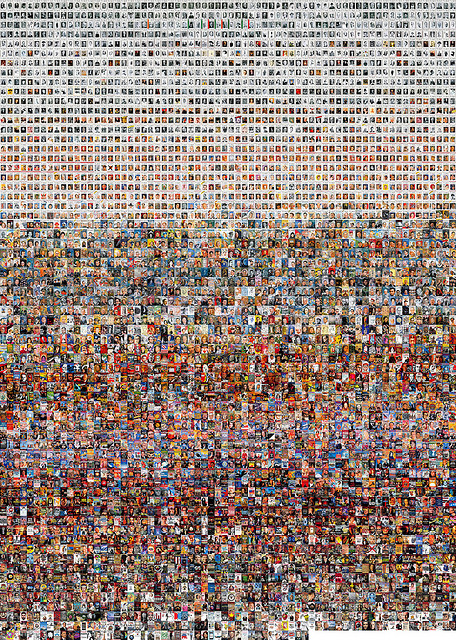
\includegraphics[width=0.5\textwidth]{time_covers}
\end{figure}


\subsection{Metadata analysis}

Images do not exist in isolation. Instead, they are surrounded by all kinds of non-visual metadata. This image metadata can be divided into a number of standard data types such as numeric, categorical, geo-spatial, and temporal, and free text. In the following we list examples from each type, deliberately mixing examples from old art held in museums and private collections, and newest form of visual art such as deviantArt artworks or amateur and professional photographs shared on Instagram, Tumblr, Flickr, 500px,, etc. 


\begin{itemize}
\item \emph{Categorical}: artists’ names, artists’ places of birth, collector’s names, auction houses, museums. 
\item \emph{Geo-Spatial}: locations of artworks, artists (when they created particular artworks), museums, users of media sharing sites, paths of visitors in museums.
\item \emph{Temporal}: dates of artwork creation; dates of their temporal trajectories 
\item \emph{Numerical}: number of likes or favorites received by artworks on social media sites; recordings of eye movements, brain activity, paths through exhibitions, or other behavior characteristics of the viewers, size of an artwork.
\item \emph{Text}: artworks titles, tags, descriptions and interpretation in art historical literature, encyclopedias, auction catalogs, comments by users of social media networks, exhibition titles, the text surrounding images that appeared as illustrations in books, the text of a web page or blog entry containing the image. 
\end{itemize}


All this metadata can be analyzed by standard graphical statistical methods developed for time series. We can summarize the data and compare the values of summaries over time; plot historical values of single variables and their combinations; analyze temporal trends using regression or time series analysis; use dimension reduction techniques such as PCA and MDS to compute distances between artworks, artists, or other entities, and see how these distances change over time. 
	In this paper, we will analyze the following metadata over time: number of subcategories, width and height of images, and their proportions, and top words used in artworks’ titles.


\subsection{Image features}
Along with the non-image metadata, we can also extract features from images and video. (To simplify the following discussion, in the following we will only consider single images.) The features are numerical summaries of different visual characteristics of images. Global features characterize these characteristics across a whole image (for example, mean brightness, saturation and hue, number of edges, etc). Local features characterize parts of images (for example, an image can be divided using a grid, and computing color and texture statistics for each part). Features are also divided into low-level, mid-level and high-level, depending on whether they describe pixel properties or semantics of the parts or whole image (faces,  types of objects, types of scenes). Some features may characterize some image characteristic using a single number, while others may consist from thousands of numbers. Another useful distinction for our discussion is between “generic features” (features originally developed for the analysis of photographs and shown to be useful for many tasks such as image retrieval and classification) and “art features” (features specifically crafted to the analysis of artworks). 
	Computer scientists normally use image features in the context of one of the standard information retrieval or data mining tasks: finding images in a database, identifying content of images, dividing them into classes based on their content, predicting the content of new images based on their features, or, more recently, automatically generating text descriptions of image scenes. There is a giant literature on what features are best to use, and new features are still being proposed - but all the discussion and practical experiments are devoted to improve computer performance on one of these tasks which do not include understanding historical evolution. And while research has shown that often the features which perform well in one task can be also successfully used in another, without experiments we can’t assume a priori that such features would also work well for the analysis of historical changes. We also can’t assume that if some features were successful for one type of visual art they would also work for other types.
	
	The use of long feature vectors consisting from thousands of features can be justified for industrial applications of common tasks such as object recognition, if the goal is efficiency and precision rather than transparency of the method (which would include intuitive understanding of the features and algorithms used). Typically scientists and their clients are happy with “black box” solutions if they offer best performance. In our case, we want our methods and their practical applications to art datasets to be meaningful to art historians, artists, museum professionals, and others who are interested in art but don’t have computer science training. The goal is to add quantitative methods to other previously developed research methods in the humanities, and not to create an efficient industry application. (Although we can imagine such applications - for example, real-time categorization of huge volume of user shared images into types, discovery of their similarity to previously shared images, real-time mapping of world’s digital visual culture, etc. For such applications, efficiency would become quite important). 


\subsection{Analysis and visualizations using extracted features}

\begin{table}[ht]
\centering
\begin{tabular}{lr}
cat.name & cat.freq \\ 
  \hline
Digital Art/000000 & 4.00\\ 
Digital Art/3-Dimensional Art & 17374.00 \\ 
Digital Art/Drawings & 30063.00 \\ 
Digital Art/Fractal Art & 34618.00 \\ 
Digital Art/Miscellaneous & 17152.00 \\ 
Digital Art/Mixed Media & 4097.00 \\ 
Digital Art/Paintings \& Airbrushing & 29394.00 \\ 
Digital Art/Photomanipulation & 29064.00 \\ 
Digital Art/Pixel Art & 4374.00 \\ 
Digital Art/Stereoscopy & 3.00 \\ 
Digital Art/Text Art & 142.00 \\ 
Digital Art/Typography & 1208.00 \\ 
Digital Art/Vector & 9087.00 \\ 
Digital Art/Vexel & 1157.00 \\ 
Traditional Art/Animations & 84.00  \\ 
Traditional Art/Assemblage & 21.00  \\ 
Traditional Art/Body Art & 2794.00  \\ 
Traditional Art/Collage & 1243.00  \\ 
Traditional Art/Drawings & 45511.00  \\ 
Traditional Art/Miscellaneous & 1880.00  \\ 
Traditional Art/Mixed Media & 6426.00  \\ 
Traditional Art/Paintings & 30209.00  \\ 
Traditional Art/Printing & 1146.00  \\ 
Traditional Art/Scratchboard & 21.00  \\ 
Traditional Art/Sculpture & 6738.00  \\ 
Traditional Art/Street Art & 4417.00  \\ 
Traditional Art/Typography & 595.00  \\ 
   \hline
\end{tabular}
\end{table}

Given this motivation, in this study we would only use a small number of global features which, in our view, are most easy to understand for non-professional audiences. Most digital camera and many camera apps include displays of color and brightness histograms. The color histograms has also been used in computer science research for two decades, so here we have a perfect match between the types of features which perform well in computational image analysis, and which are also familiar to wide audiences. We will use full 256 bin HSV histograms to calculate distances between single images and categories in feature space, project this space into two dimensions using PCA, and visualize positions of category centers over the years. For the plots showing how single image characteristics change over time, we will use values of H,S.V features averaged per category and per year.
The reliance of perceptually meaning features is ideal, but it also risks missing important patterns of visual changes if they can’t be captured with these features. In our analysis, we will use a variation on on single “non-intuitive”  feature already shown to perform well in other image tasks - size of compressed jpeg image in kb. We will normalize this size by number of pixels in an image. Similar to image entropy measurement, compressed image size indicates image complexity and presence of details. 
We experimented with comparing individual deviantArt artists by plotting average values of single global features (such as mean brightness) versus average standard deviations of these same features for all artist’s artworks. We discovered that such simple plots characterize well artist’s stylistic diversity (or sameness). If all artworks of a given artist have a narrow range of global feature values, this indicates that the artist has a well-defined style. conversely, a big spread in values of global features indicate that the given set artworks does not follow a narrow style. In this paper, this technique will be applied to larger categories containing many images. We will calculate standard deviations of brightness mean and standard deviations of pixel values per image, average them for all images in a category, and then plot these averages over time. 
We introduce another method for visualizing temporal development in visual art - plots of pairwise time distances. XXXX


\subsection{Pairwise Distance Correlation between Color Features and Years}

Here we present a method, that we call Pairwise Distance Correlation, for measuring the change of colors of images over time. This method is closely related to \cite{lamport94}, but we introduce the notion of learning the distance metric from data using a Quadratic Program (QP). Our approach is as follows: consider a set of $N$ features and targets $\{ (f_{1}, t_{1}), \ldots, (f_{N}, t_{N})\}$. Here the features $f_{i} \in \Re^{n}$ are the color features we described above for each year $t_{i} \in \Re$ $\forall i \in (1, \ldots, N)$. We propose that if there is a relationship between features $f_{i}$ and targets $t_{i}$, then this relationship should also be preserved between the distances of pairs of features $(f_{i}, f_{j})$ and pairs of targets $(t_{i}, t_{j})$. Put another way, if there is a relationship between color features and time, then $\exists \epsilon, \delta$ such that $\|f_{i} - f_{j} \| \le \epsilon$ and $\|t_{i} - t_{j}\| \le \epsilon$ for $|i - j| \le \delta$. Note that this only hold true if the distance between features from years that are farther apart should be larger than the distance between features from years that are close. Effectively we can test this by measuring the correlation between $\|f_{i} - f_{j}\|$ and $\|t_{i} - t_{j}\|$.

Measuring the correlation between $\|f_{i} - f_{j}\|$ and $\|t_{i} - t_{j}\|$ relies on the assumption of choosing an appropriate distance metric. To generalize the metric, we propose using a weighted 2-norm $\|f_{i} - f_{j}\|^{2}_{W} = (f_{i} - f_{j})^{T}W(f_{i} - f_{j})$ where the weighting matrix $W \in S_{++}^{n \times n}$ (this is to ensure that we are still using a proper metric) is learned from data. Here, to learn the weighting matrix, we consider the special case of having only a diagonal weighting matrix, that is $W = \text{diag}(w_{1}, \ldots, w_{n})$ and $w_{k} \ge 0$ for $k = 1, \ldots, k$. To learn the optimal weighting matrix from our data set, we solve the following optimization problem:

\begin{equation} \label{eq:opt_src} 
\begin{aligned}
& \underset{W}{\text{minimize}} & & \sum_{i,j} \big(\|f_{i} - f_{j}\|^{2}_{W} - (t_{i} - t_{j})^{2}\big)^{2}  \\
& \text{subject to} & & W = \text{diag}(w_{1}, \ldots, w_{n}) \\
& & & w_{k} \ge 0, \; k = 1, \ldots, n.
\end{aligned}
\end{equation}
The objective function in Equation \ref{eq:opt_src} is the sum of squares of differences between $\|f_{i} - f_{j}\|^{2}_{W}$ and $(t_{i} - t_{j})^{2}$ for all $(i,j)$ feature and target pairs in the data set. Thus, for the data set of $N$ examples, there are $N(N-1)/2$ terms in the summation. The optimization problem in Equation \ref{eq:opt_src} We are seeking the weighting matrix $W$ that minimizes this objective function while satisfying the constraints. Note that we can simplify $\|f_{i} - f_{j}\|^{2}_{W}$ as

\begin{equation*}
\begin{aligned}
\|f_{i} - f_{j}\|^{2}_{W}  &= (f_{i} - f_{j})^{T}\text{diag}(w_{1}, \ldots, w_{n})(f_{i} - f_{j})\\
& = (f_{i} - f_{j})^{T}\text{diag}(f_{i} - f_{j})w
\end{aligned}
\end{equation*}
where $w = (w_{1}, \ldots, w_{n})^{T}$. We can write Equation \ref{eq:opt_src} equivalently as 

\begin{equation} \label{eq:opt_src} 
\begin{aligned}
& \underset{w}{\text{minimize}} & & \sum_{i,j} \big((f_{i} - f_{j})^{T}\text{diag}(f_{i} - f_{j})w - (t_{i} - t_{j})^{2}\big)^{2}  \\
& \text{subject to} & &  w_{k} \ge 0, \; k = 1, \ldots, n. 
\end{aligned}
\end{equation}

\subsection{Dataset}

This section we are going to discuss the data set at great length:



\section{Results}

We have analyzed both selected metadata available for 270,000 art images created by users of DeviantArt.com between 2000 and 2010, and color features of these images. There is no apriri reason to expect that neither subject matters nor visual characteristics changes in any systematic way in these images over this period. But if there was any changes, we may expect to find it in Digital Art rather than Traditional Art - while the tools and techniques used to make art in the latter category have not changed for many decades, digital tools and platforms (i.e. software such as Photoshop and Painter, and hardware such as desktops, laptops and later in the decade tablets) were rapidly developing in 2000-2010. Computers were getting faster, resolution and the size of RAM were increasing, and storage was getting cheaper, allowing people to create high-resolution images with more complex effects.

The results of our analysis were very suprizing. While some aspects of images in Digital Art category did change during the study period, these changes were relatively small. However, images in Traditional Art category changed in a systematic way during this period, and the amount of these changes was much larger than for Digital Art. Our analysis also revealed other interesting differences between Digital Art and Traditional Art, which were not previously noted by by any art historians or digital media scholars.  In this section, we will go through details of our analysis. We start with qualitative and quantitative aspects of the category system: growth in the number of images in Digital and Traditional Art, gradual development of hundreds of sucategories, and changes in image proportions and sizes (in pixels). Next, we discuss changes in color features we extracted from all images in our dataset, and compare these changes for Digital Art vs. Traditional Art.

\subsection{Metadata}

\subsubsection{Categories} DeviantArt.com started in August 2000. Since the beginning, the number of top-level categories and subcategories systematically grew to accomodade variety of techiques and subjects in artworks submitted by the site users. The category system is organized as a tree, with a number of top-level categories (including Traditional Art and Digital Art) containing further subcategories. By 2011, many "brunches" of this tree had up to 6 levels of sub-categories under them, and the total number of all subcategories was over 1700. Examining the structure of this category tree, we see that first and second level divide art into different media: for example, XXX/XXX or XXX/XXX. Subequent sub-categories often describe subject matter of artworks: for example, XXX/XXX/XXX or XXX/XXX/XXX. Overall, we have a very detailed encyclopedic picture of contemporary creativity, reflecting contributions and interests of millions of artists. This very detailed category system is one of the most valuable and unique features of DeviantArt.com network, because it does not exist in the same organized form anywhere else. The analysis of the historical development of the categories structure offers us a unique way to understand how popular art developed during the first decade of the 21st century.  

In our analysis, we compared the numbers of all subcategories for Traditional Art and Digital Art over the years. While these numbers systematically grew over the years for both categories, this growth was creating twice as many subcategories within Digital Art vs. Traditional Art. By the end of 2001, Traditional Art had 10, while Digital Art had 22; in 2005, these numbers were 81 and 162; in 2010, there were 113 and 216. Separately from comparing the total number of subcategories created over the years, we can also examine how many of these subcategories were active (i.e, user or users contributed at least one new image in a given subcategories) at any given day, or any temporal unit. Fig. XXX show the numbers of active subcategories in Traditional and Digital Art per day from 2000 to 2010 for one image sample. While the numbers are smaller than the total number of all subcategories created (not every subcategory was receiving a new image daily), we see the same pattern: the numbers of active subcategories for Digital Art are systematically larger than the numbers for Traditional Art. Comparing the total number of images placed by users within these two categories once again confirms the same pattern: our sample contains 101,085 images in Traditional Art category, and 177,737 in Digital Art category.
    
What are the reasons for this strong difference? Examining the names and organization of subcategories suggests the following explanation. Both categories have many sub-categories describing the techniques or tools used to create art, and this number is significantly bigger for Digital Art. The examples of such subcategories in Traditional Art are xxx, xxx, and xxx; the examples of subcategories in Digital Art are XXX. [We created an interactive visualization which can be used to examine all subcategories in our dataset: URL ]  [ADD MY EXPLANATION]
    

[Desired: some quantitative measure of difference between number of active categories in Digital Art vs Traditional Art] 

 
\begin{figure}
    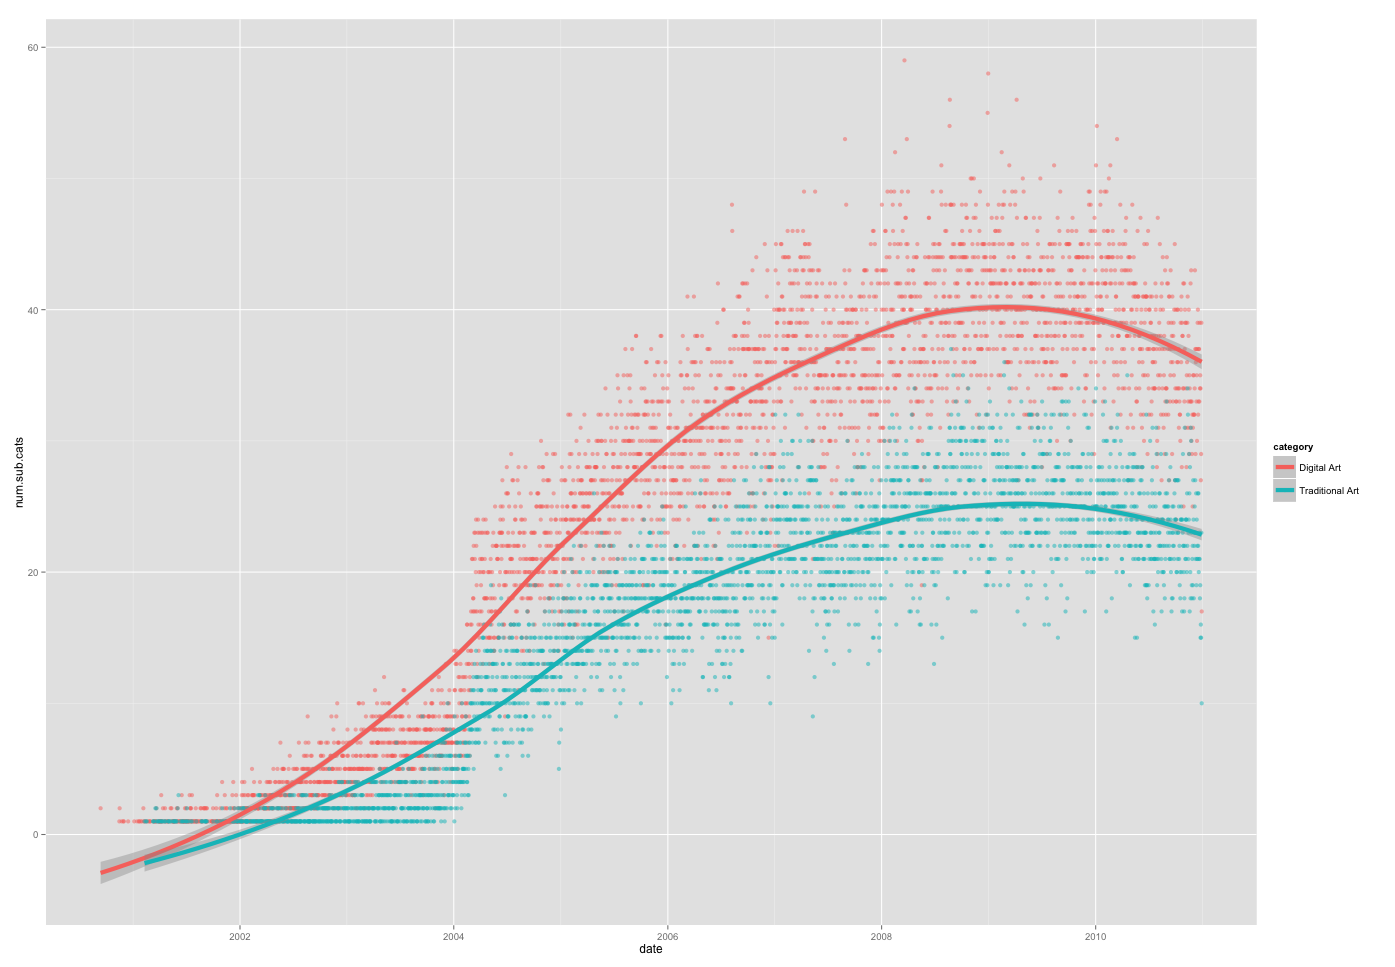
\includegraphics[width=0.5\textwidth]{active_categories_per_date}
    \caption{Number of Active Categories Per Day}
\end{figure}


\subsubsection{Images sizes and proportions} As we already noted above, given the systematic changes in software and hardware for digital art creation, we can expect that this will be reflected in Digital Art images characteristics, with images getting progressively larger (as measured in pixels horizontally and vertically).In the case of Traditional Art, while the art tools for its creation did not change, the mechanisms for moving this art into the web did evolve. Until 2008-2009 when smart phone cameras acquired suitable resolution for taking photos of artworks, its safe to assume that DeviantArt.com contributors used flatbed scanners to scan their artworks. [ADD SOME DETAILS?] Unfortunately, we don't have image header information which could have told us these details.[SOMETHING ABOUT PRICES OF DIGITAL SCANERS?] Additional interesting characteristic which can be analyzed is the proportion between width and height. While both Traditional Art and Digital Art have portraits and landscapes subcategories, they contain only a small proportion of total images. Therefore, we did not have any particular expectations about image ratio, not did we had reasons to expect that they will be different for Traditional and Digital Art.

The analysis of images sizes and proportions also led to suprizing findings, which can't be related to any a priori quantitative art historical or media theory researh. Fig XXX plots width and height (in pixels) for all images in our dataset, (with the few outliers excluded.) Each image is represented by a point The smooth curve which acts as the border for a combination of width and height is the result of the deliberate limitation in DeviantArt web site which prohibits users from adding images bigger than a particular size - so this is not an interesting finding. But the big difference between clustering of points for Traditional and Digital Art is. While the sizes for Digital Art vary free, a larger proportions of sizes for Traditional Art concentrate along a small number of widths and heights. We propose the following explanation for this interesting patterns. When a user of Painter, Photoshop, 3D Studio Max or any other digital software program for photo-editing, painting and drawing or 3D design creates a new image, s/he can easily choose any size. Equally importantly, at any time during creation process, s/he can very easily crop the image or add new area. Each operation requires just a few clicks. But the artworks in Traditional Art category typically begin with physical materials bought in art store, such as canvases and paper. These materials are sold in a fixed number of sizes and proportions. And while it is certainly   


[ Include table that shows the average image ratio and image area for each year for digital and trad category ]

\begin{figure}
    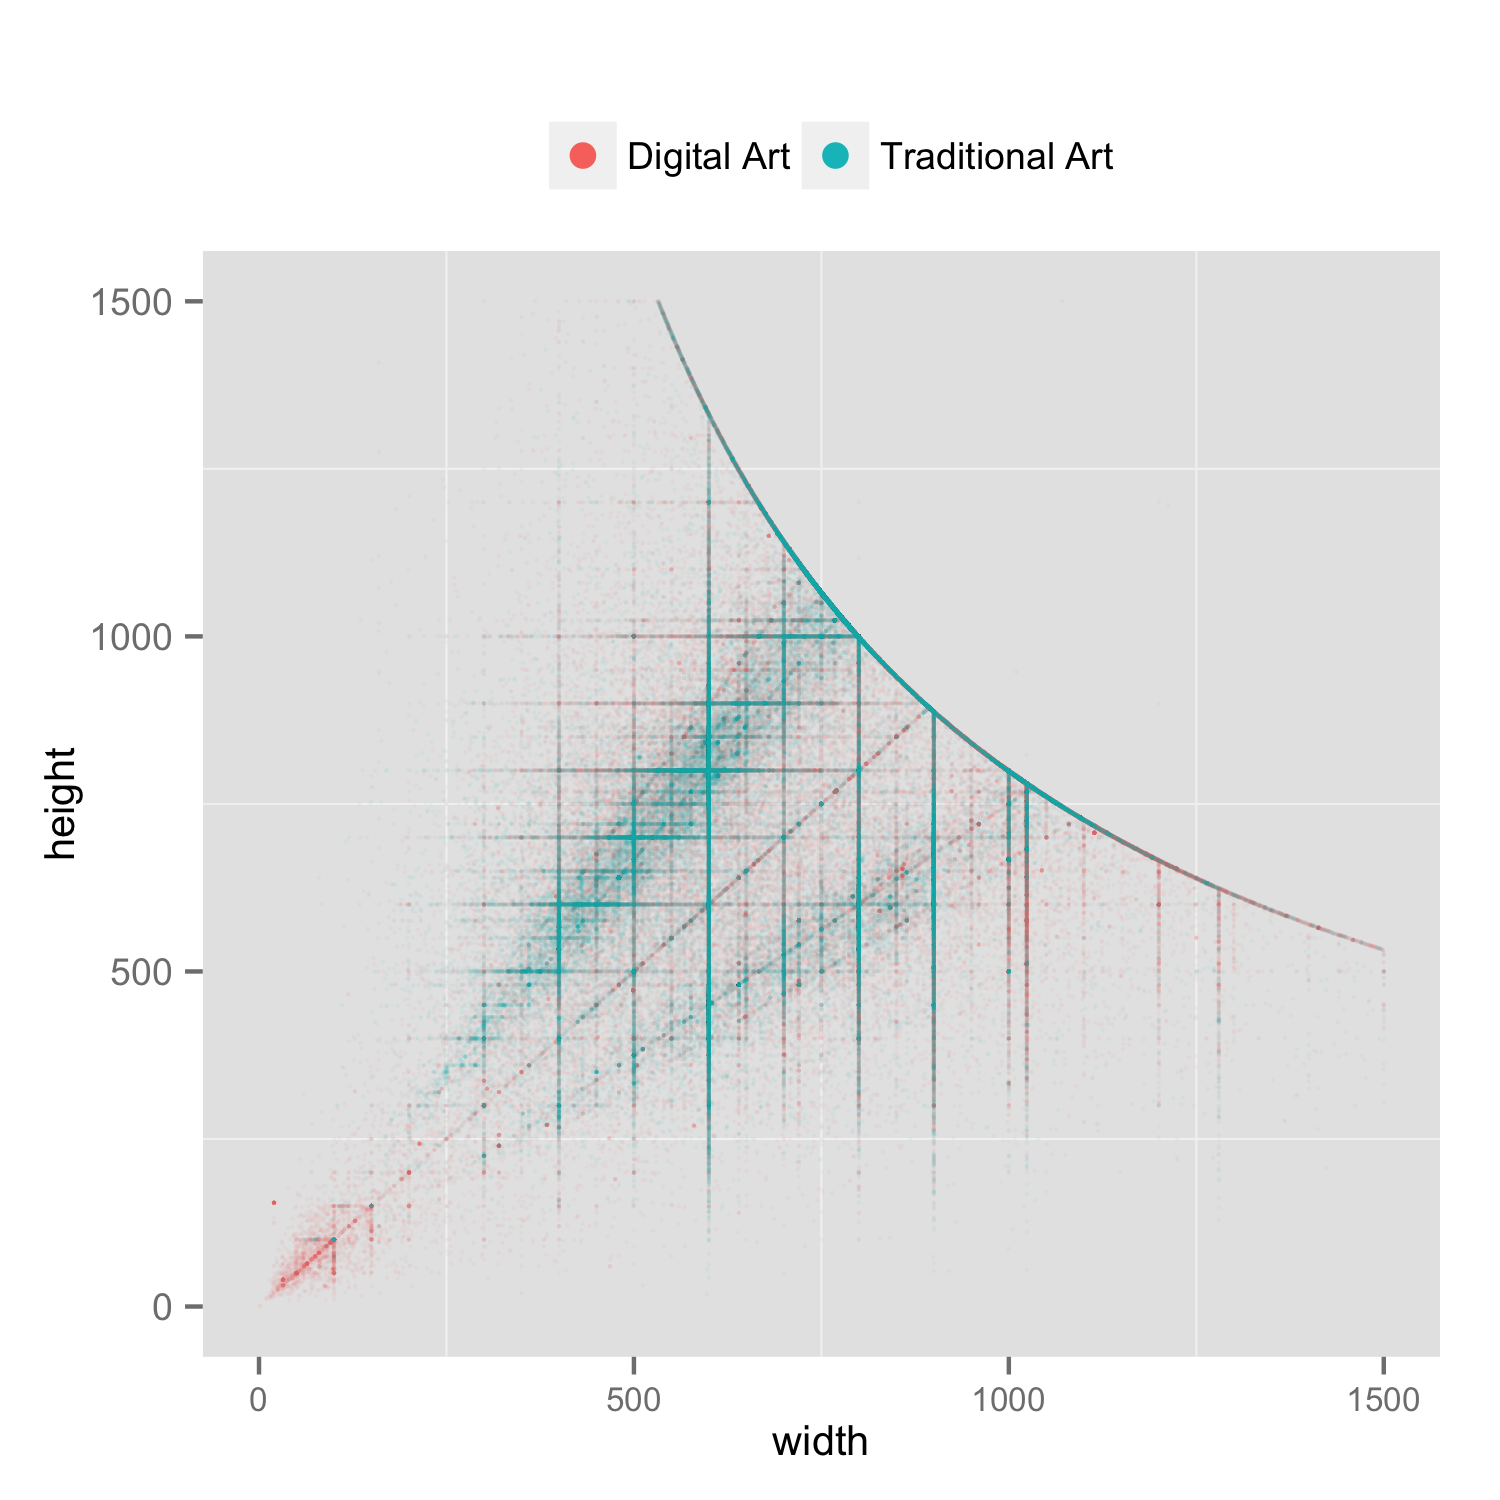
\includegraphics[width = .5\textwidth]{width_height}
  \caption{Image Width by Height}
\end{figure}


\subsection{Image Features} In this section we extract HSV features from the artworks and measure the temporal evolution of Digital Art and Traditional Art between the years 2001 and 2010. These features include the mean and standard deviation (STD) of the Hue, Saturation and Value of each image. Using these features, we discuss simple yearly summary statistics to measure the change of HSV. In addition, to capture a richer set of features for color, we also extract the XXX-bin histograms of the Hue, Saturation and Value. We use Principle Component Analysis of these HSV histograms to visualize the yearly change of HSV features for Digital Art and Traditional Art. Finally, we introduce a novel method inspired by the distance correlation statistic to measure the yearly changes in HSV for images. 

\begin{figure}
    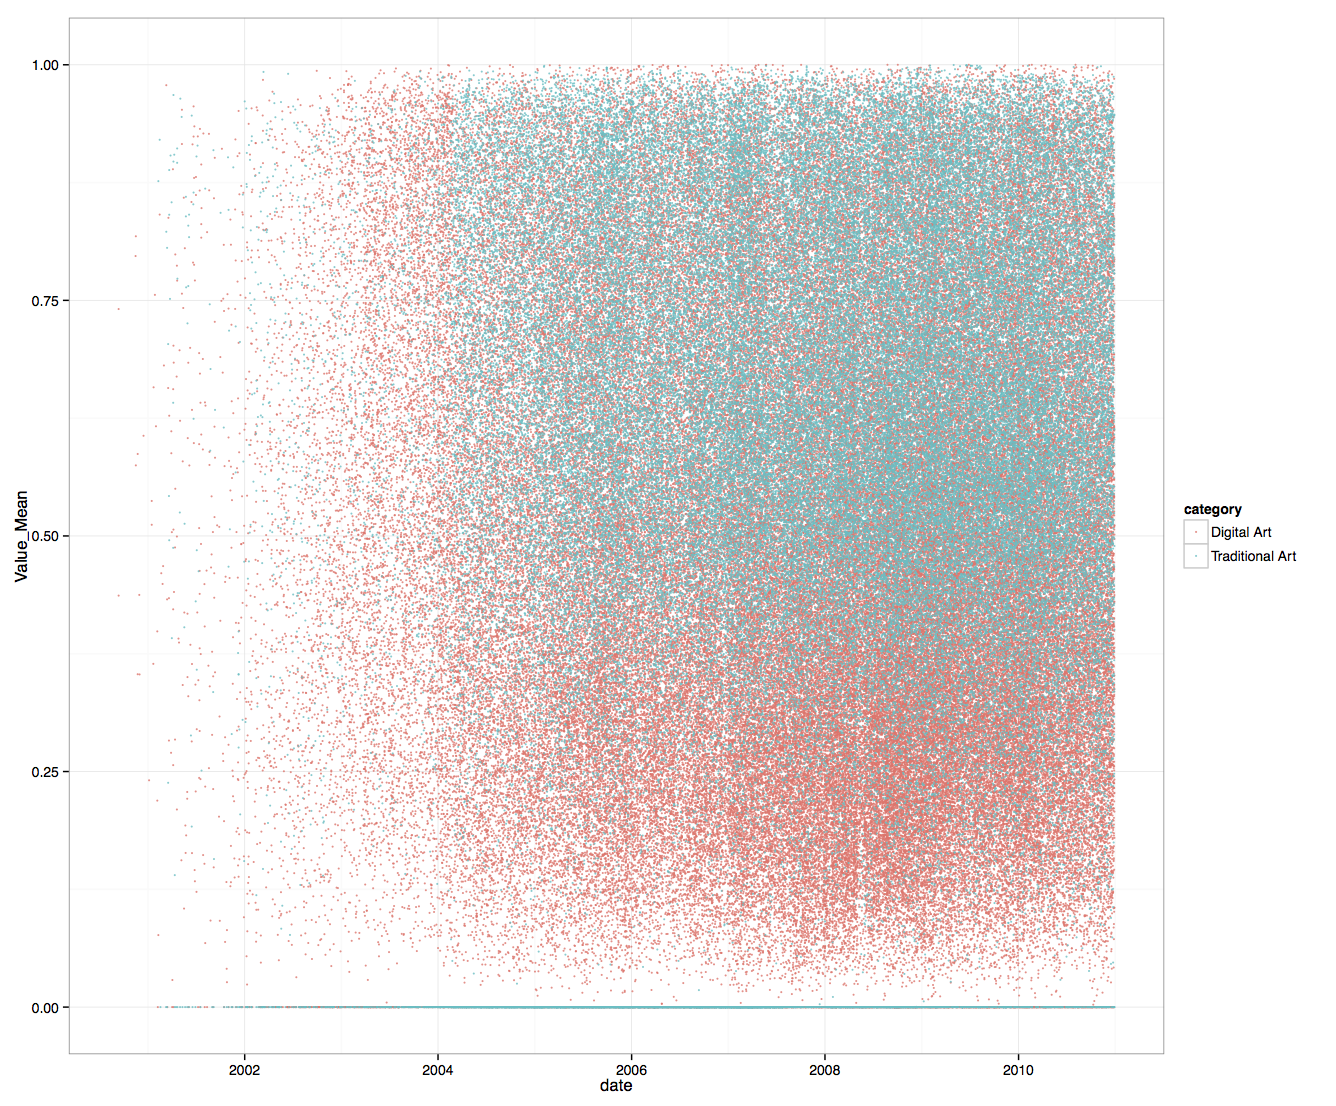
\includegraphics[width=0.5\textwidth]{value_mean_per_image_over_dates_PNG}
    \caption{Mean Grayscale Value of Images Over Time}
    \label{fig:MeanGrayScale}
\end{figure}

\subsubsection{Aggregates} In Figure ~\ref{fig:MeanGrayScale} we show the scatter plot of the average Value (equivalent to gray-scale value of the image) for each artwork in our data set. This figure illustrates that Traditional Art has much more narrow distribution of gray-scale values than Digital Art. Similarly, Figure ~\ref{fig:MeanHSV_yearly} shows the mean HSV and standard deviation of HSV aggregated using a simple average for each year. As in Figure ~\ref{fig:MeanGrayScale}, we see that the distribution of gray-scale values in Figure ~\ref{fig:MeanHSV_yearly} (middle panel) for Traditional Art is tighter than for Digital Art. The average distribution of Saturation levels for Digital Art and Traditional appear to be quit different, although we see that by 2010 the standard deviation of traditional art approach that of digital art. However, the distribution of Hues (left panel of Figure ~\ref{fig:MeanHSV_yearly}) appears that the distribution of Hues for Digital Art and Traditional Art are very similar. 

\begin{figure}
    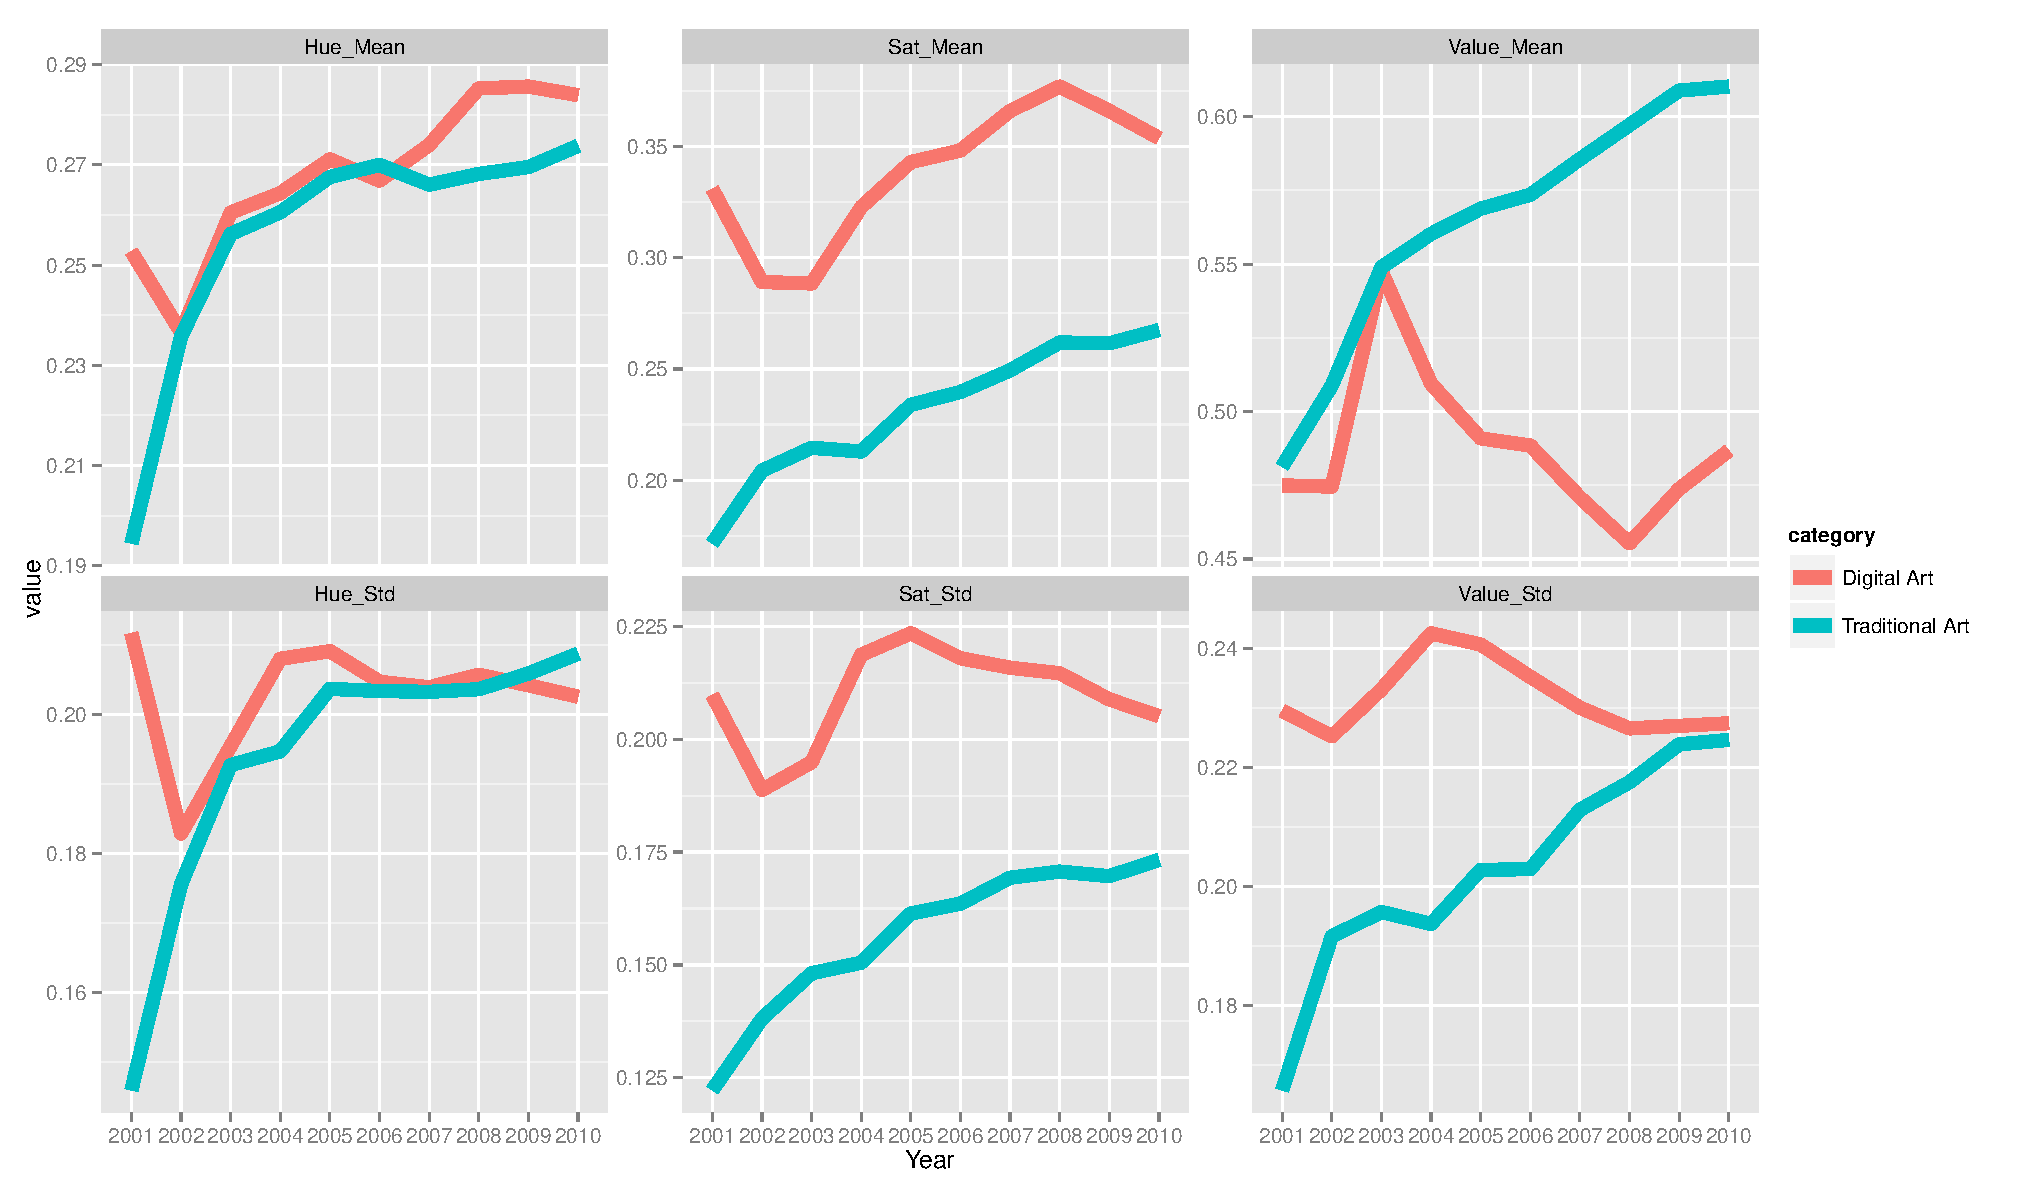
\includegraphics[width = .5\textwidth]{hsv_time_2_cat}
      \caption{Average HSV Features per Year}
     \label{fig:MeanHSV_yearly}
\end{figure}

Figure ~\ref{fig:MeanHSV_yearly} suggests that HSV characteristics of both Digital and Trditional Art Simp

Since these results are based on simple summary statistics of the Hue, Saturation, and Value distributions, we suspect that a great deal of details is being washed out and therefore Figures ~\ref{fig:MeanGrayScale} and ~\ref{fig:MeanHSV_yearly} are both misleading. 

\subsubsection{Principle Component Analysis}
To extract colour features at a finer resolution, we also extract XXX-bin Hue, Saturation, and Value histograms for each image. We then compute the average HSV histograms for each year and normalize each bin component with the standard deviation of each component. To visualize this feature set, we use Principle Component Analysis (PCA) to project the feature vectors into a two-dimensional subspace. Figure~\ref{fig:Hpca} shows the top two Principle Components of PCA for the Hue distributions. This figure shows that Digital Art primarily varies along the second PC. Traditional Art, on the other hand, varies a great deal along both the first and second PC. 

\begin{figure}
    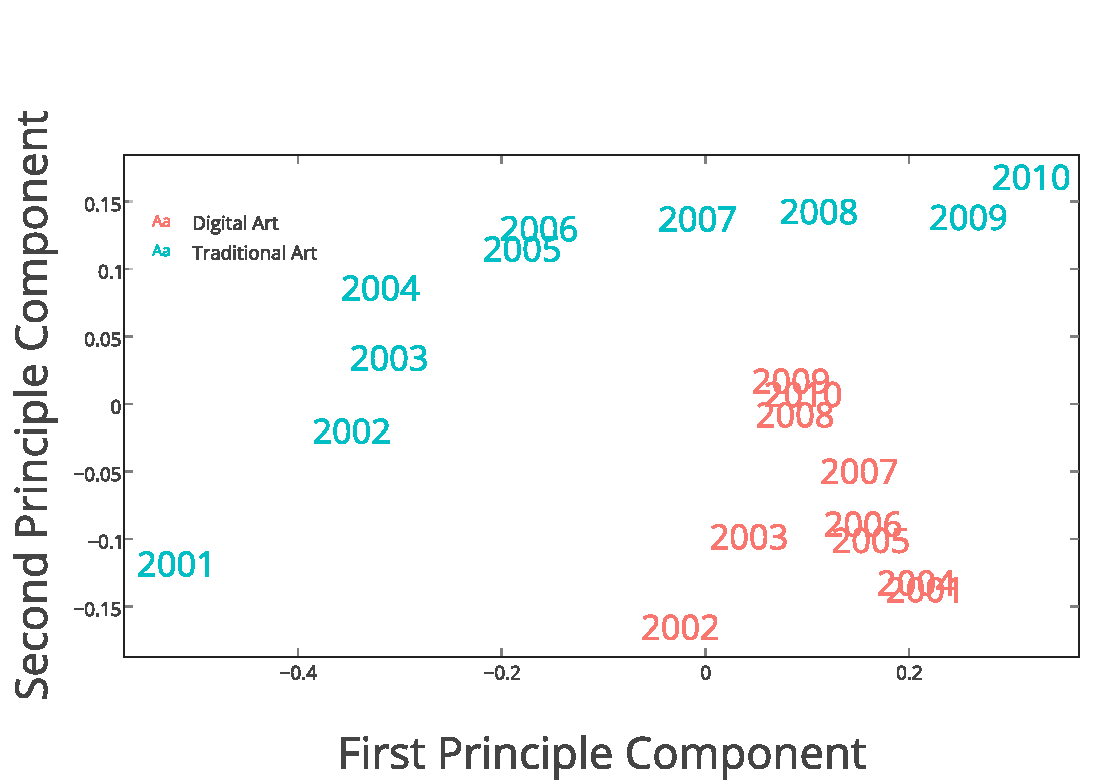
\includegraphics[width = .4\textwidth]{pca_hue}
  \caption{PCA Hue}
  \label{fig:Hpca}
\end{figure}


This suggests that the color distribution of Traditional Art varies more than Digital Art. Furthermore, the PCA suggests that Traditional Art has two primary ``phases." Before 2005, the majority of variance for Traditional Art is along the second PC. After 2005, the majority of variance for Traditional Art changes from the second PC to the first PC.  Digital Art does not exhibit such phases. In fact, from Figure ~\ref{fig:Hpca} it appears that Digital Art does not have an orderly temporal structure as Traditional Art does. To quantify  these temporal difference and correlation, we use the distance correlation in the next section.


\subsubsection{Distance Correlation} Here we discuss using correlation distance to measure the temporal changes of Hue, Saturation, and Value for artworks. Figure \ref{fig:pair_diff} shows a scatter plot of the pairwise distances between the average Hue histogram distributions for every year for the Digital Art and Traditional Art categories. This figure shows that as the difference in the number of years increases, the distance between the Hue distributions also increases. Furthermore, we see that the differences in Hue distributions for Traditional Art are significantly greater than for Digital Art. In other words, the changes in Hue distributions of Traditional Art images from the late 2000's relative to the early 2000's are much larger than for Digital Art. 


\begin{figure}
    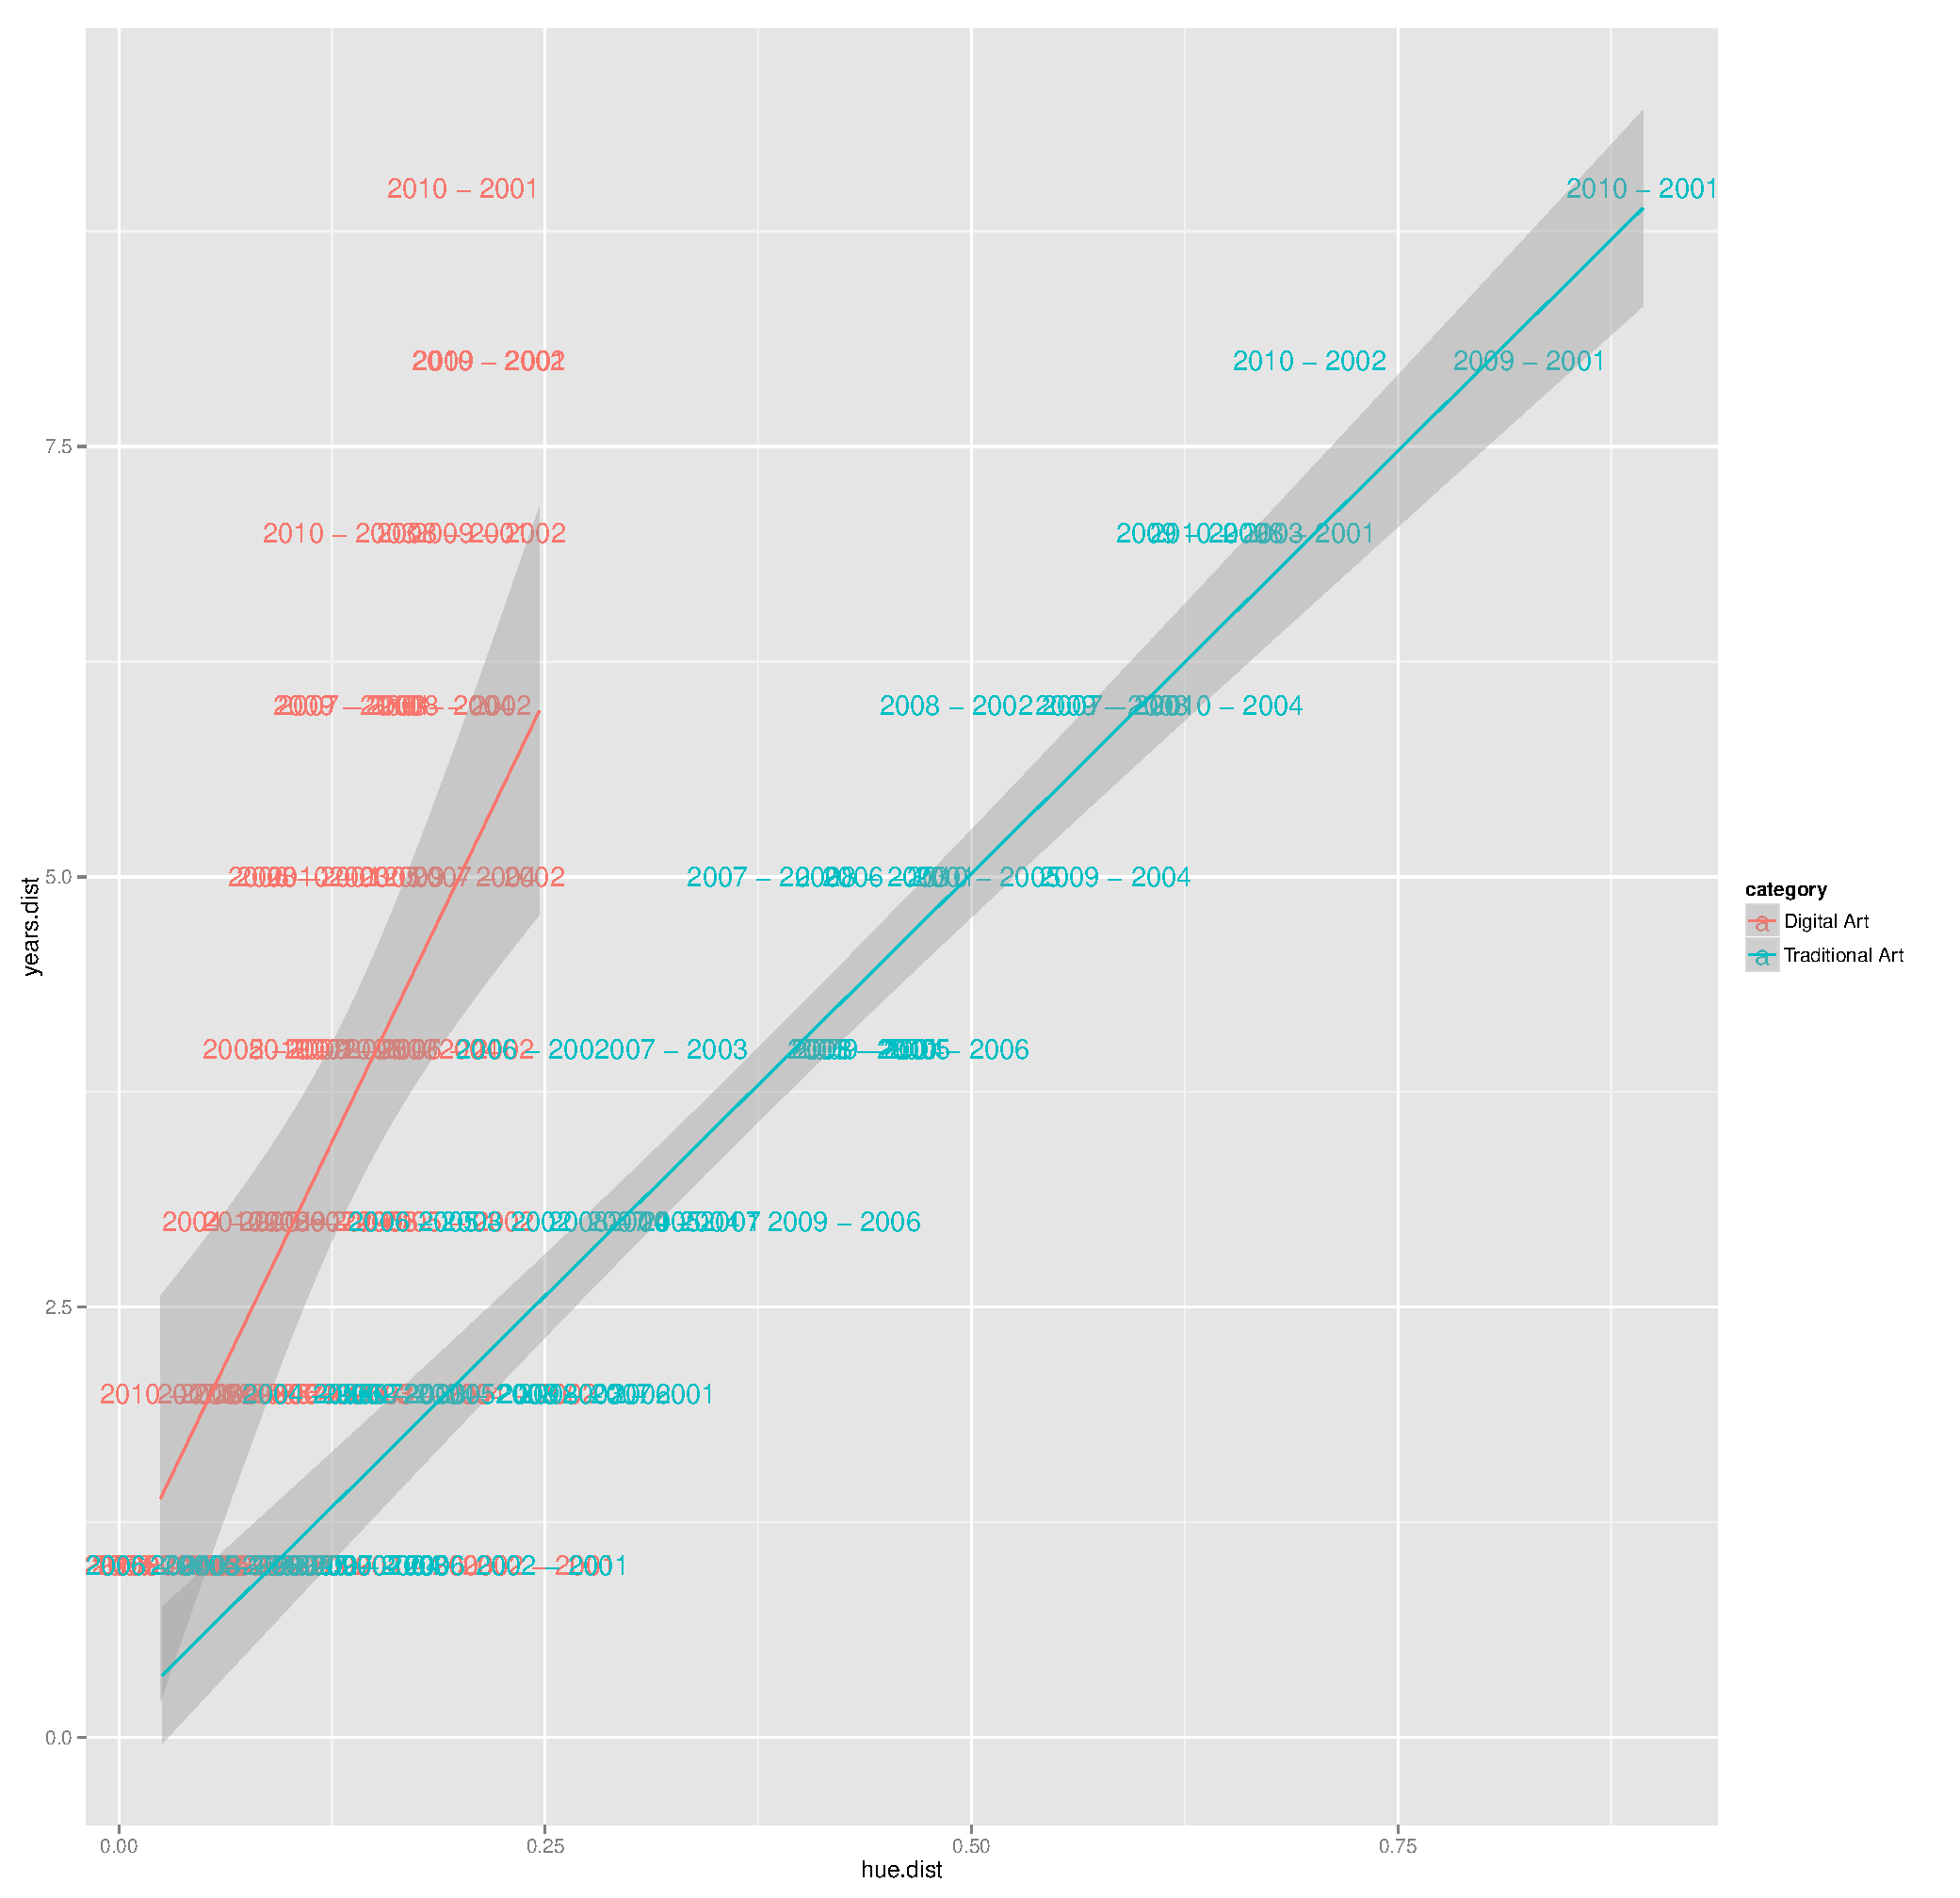
\includegraphics[width = .4\textwidth]{Hue_time}
  \caption{Change of Hue over Time}
  \label{fig:pair_diff}
\end{figure}

\begin{figure}
    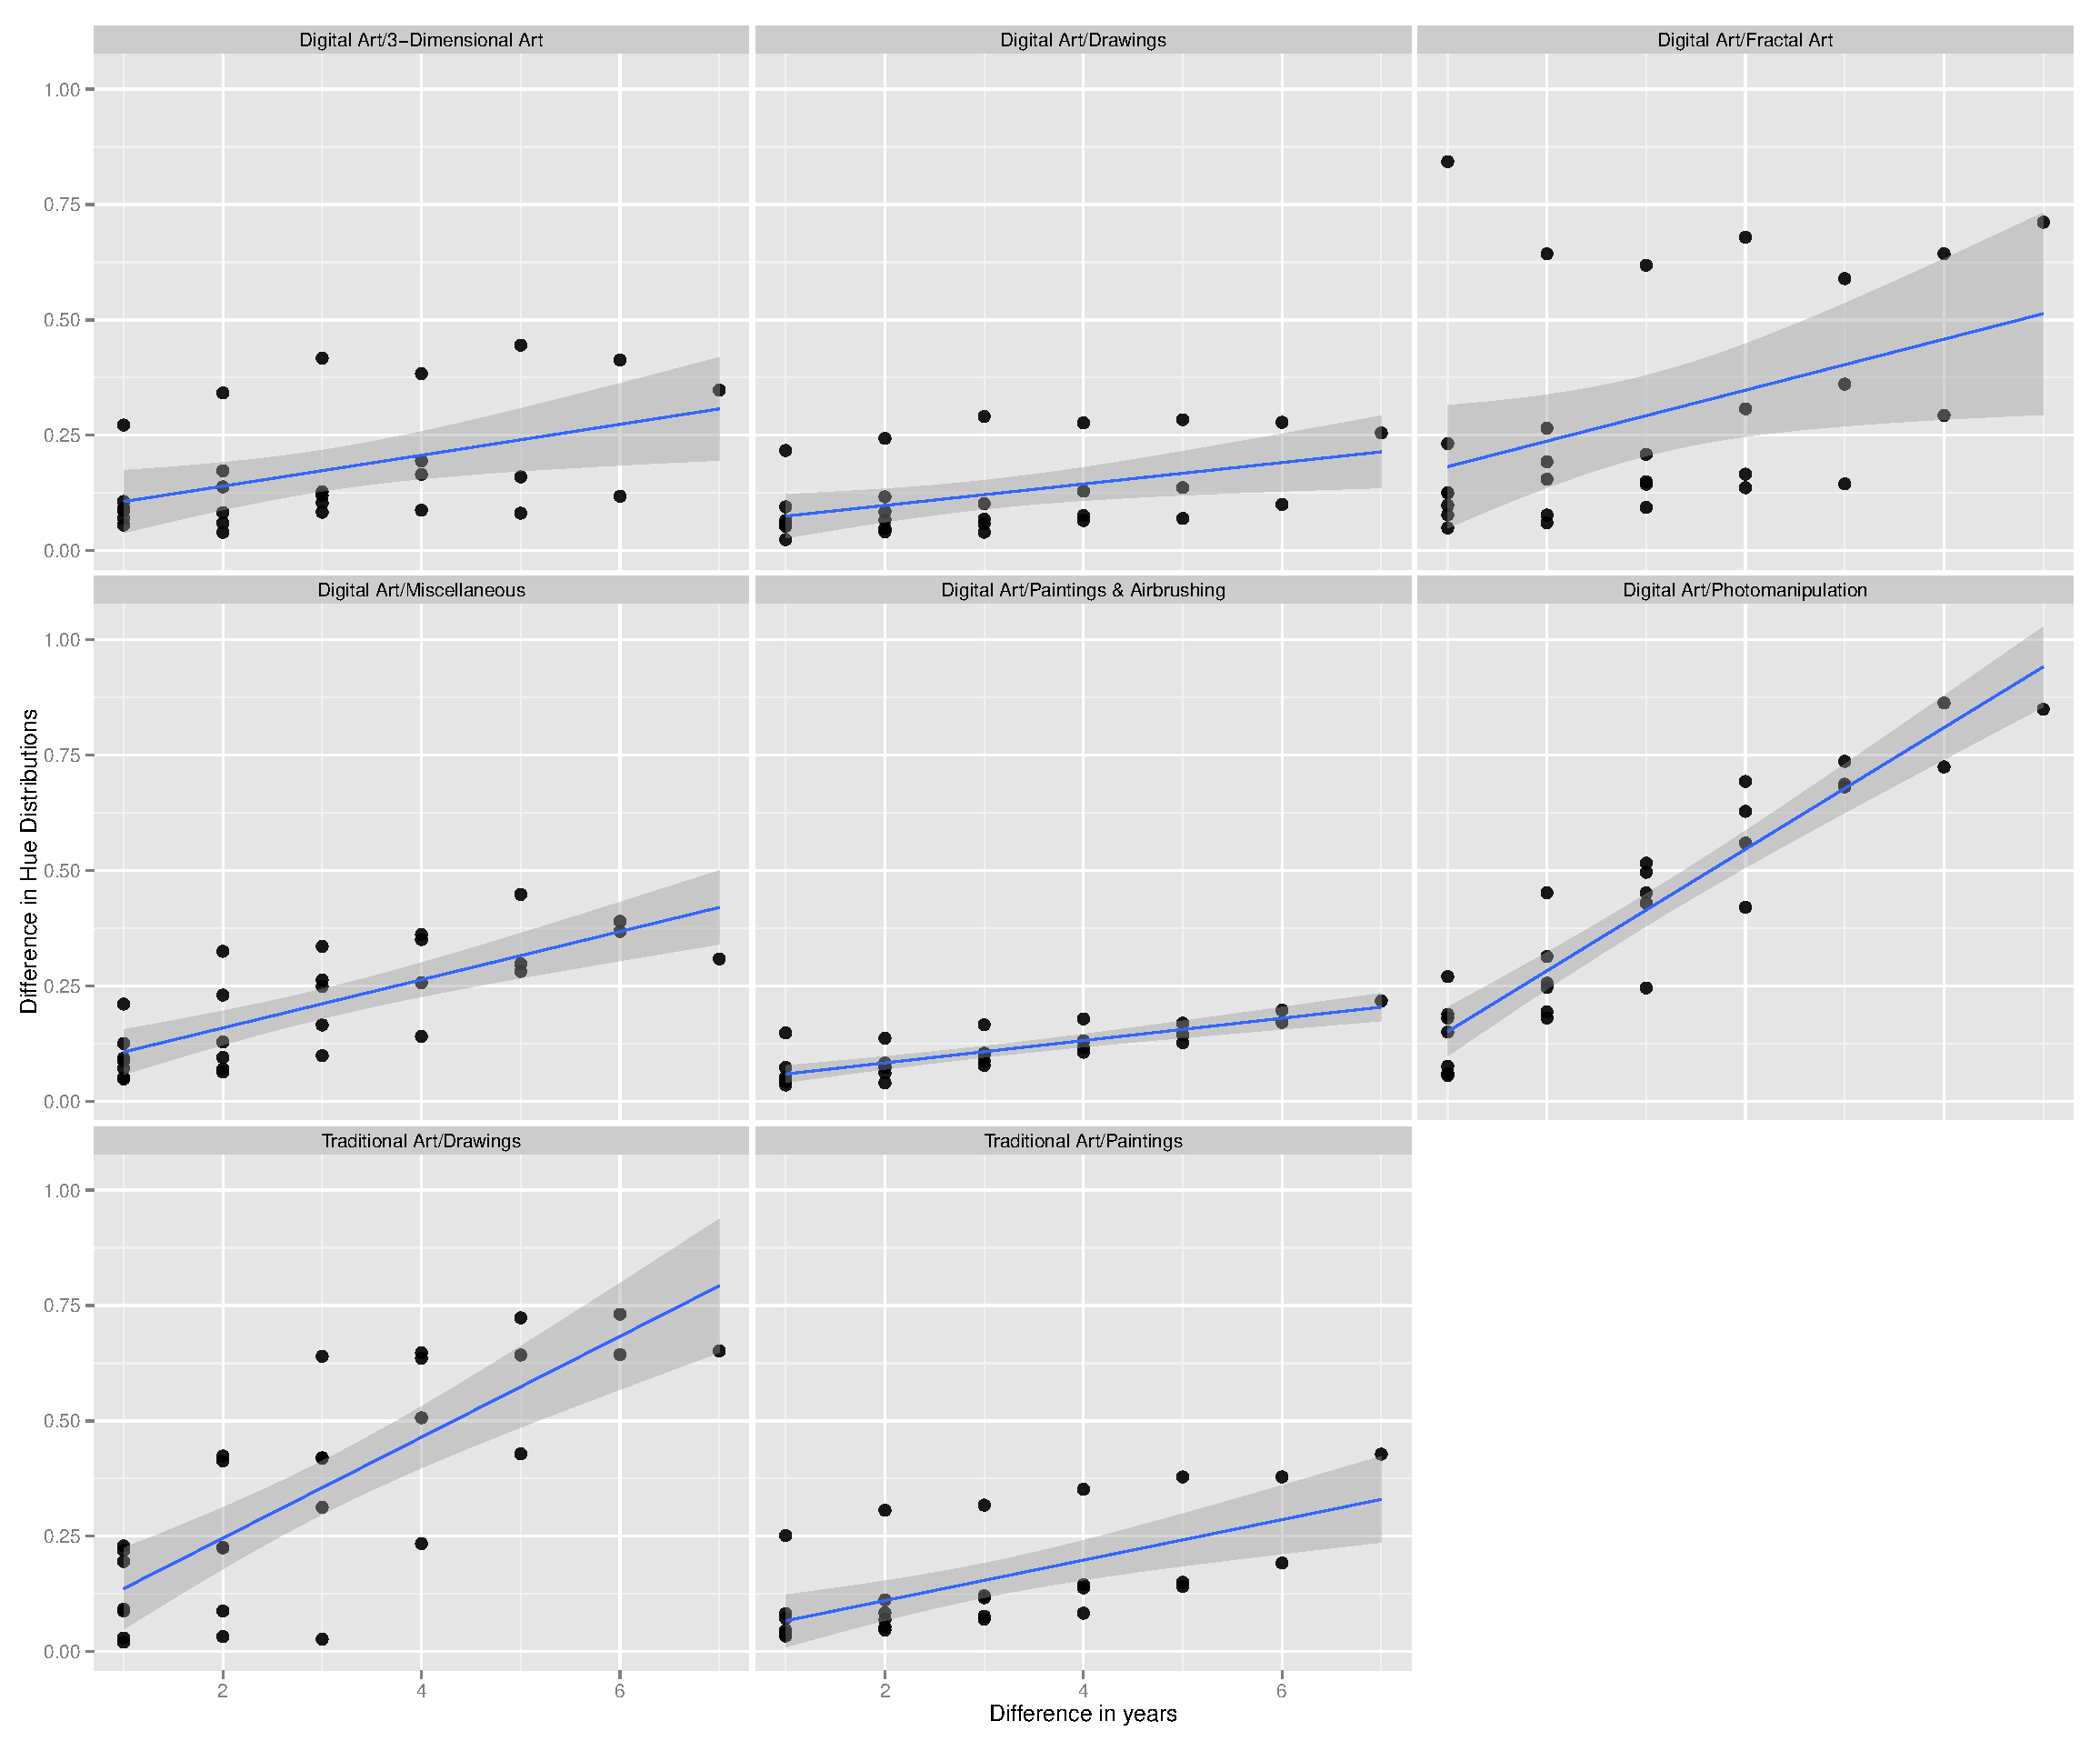
\includegraphics[width = .4\textwidth]{Hue_time_sub_cats}
      \caption{Change of Hue over Time for subcategories}
    \label{fig:pair_diff_subcat}
\end{figure}


\begin{thebibliography}{9}

\bibitem{lamport94}
  Leslie Lamport,
  \emph{\LaTeX: a document preparation system}.
  Addison Wesley, Massachusetts,
  2nd edition,
  1994.
 
\end{thebibliography}

\end{document}
